\chapter{Videospiele}

Bei Videospielen handelt es sich um interaktive Medien, die Spielern eine immersive und unterhaltsame Erfahrung bieten. Sie erm�glichen eine Interaktion zwischen einem Spieler, einer Hardware und gelegentlich weiteren Spielern. Diese Interaktion erfolgt mithilfe von Eingabeger�ten in einer fiktionalen Spielwelt. Bei den Eingabeger�ten kann es sich um eine Maus, Tastatur, Gamepad oder Touch-Display handeln. Die fiktionale Spielwelt wird �ber die Ausgabeger�te der Hardware visuell, akustisch oder haptisch simuliert. Innerhalb des Videospiels wird der Spieler durch seine Handlungen und Konsequenzen emotional beeinflusst. \autocite{Bergonse}

\section{Perspektiven}

Nicht nur Filme und Literatur, sondern auch Videospiele werden von ihrem Nutzer �ber eine Perspektive erfasst. So werden Filme �ber verschiedene Kameraperspektiven gedreht, die auch in Videospielen vorhanden sind. In Videospielen spricht man von den folgenden Perspektiven: Third-Person und First-Person.

Die Third-Person-Perspektive ist eine Perspektive au�erhalb der gesteuerten Spielfigur und kommt in 2D und 3D Umgebung sowie in allen Genres vor.

Das Gegenst�ck zu der Third-Person-Perspektive ist die First-Person-Perspektive, die auch als Egoperspektive bezeichnet wird. Bei dieser handelt es sich um eine Perspektive aus den Augen der Spielfigur.

\section{Genres}

Genres kategorisieren k�nstlerische Werke nach ihren Eigenschaften, wie nach ihrem Inhalt und ihrer Art. Sowohl Filme, Musik und Literatur als auch Videospiele z�hlen zu k�nstlerischen Werken. So lassen sich Videospiele nach ihrem Spielinhalt und ihrer Spielart unterteilen. Klassische Videospiel-Genres sind Renn-, Rollen-, Strategiespiel, Horror und Shooter. Ein Videospiel muss nicht ausschlie�lich einem Genre angeh�ren, sondern kann auch mehreren Genres zugeordnet werden. So f�llt das Videospiel F.E.A.R First Encounter Assault Recon in die folgenden beiden Genres: Horror und Shooter.

Videospiel-Genres werden wiederum durch Subgenres nach ihren Darstellungen, Perspektiven und Spielmechaniken unterteilt. So k�nnen Videospiele des Genre Shooter entweder in der 2D oder 3D Umgebung spielen. Je nach Perspektive wird ein Shooter entweder als Third-Person-Shooter (TPS) oder als First-Person-Shooter (FPS) bezeichnet. Spielmechaniken beeinflussen die Spielweise des Videospielers. Unter anderem gibt es Spielmechaniken, die dem Spieler die M�glichkeit geben, K�mpfe durch Schleichen zu vermeiden. Shooter mit dieser Spielmechanik werden als Stealth-Shooter bezeichnet. Im Gegensatz zum Stealth-Shooter zwingt der Action-Shooter den Spieler aktiv zum Kampf, wie im Videospiel F.E.A.R.

\begin{figure}[h]
  \centering
  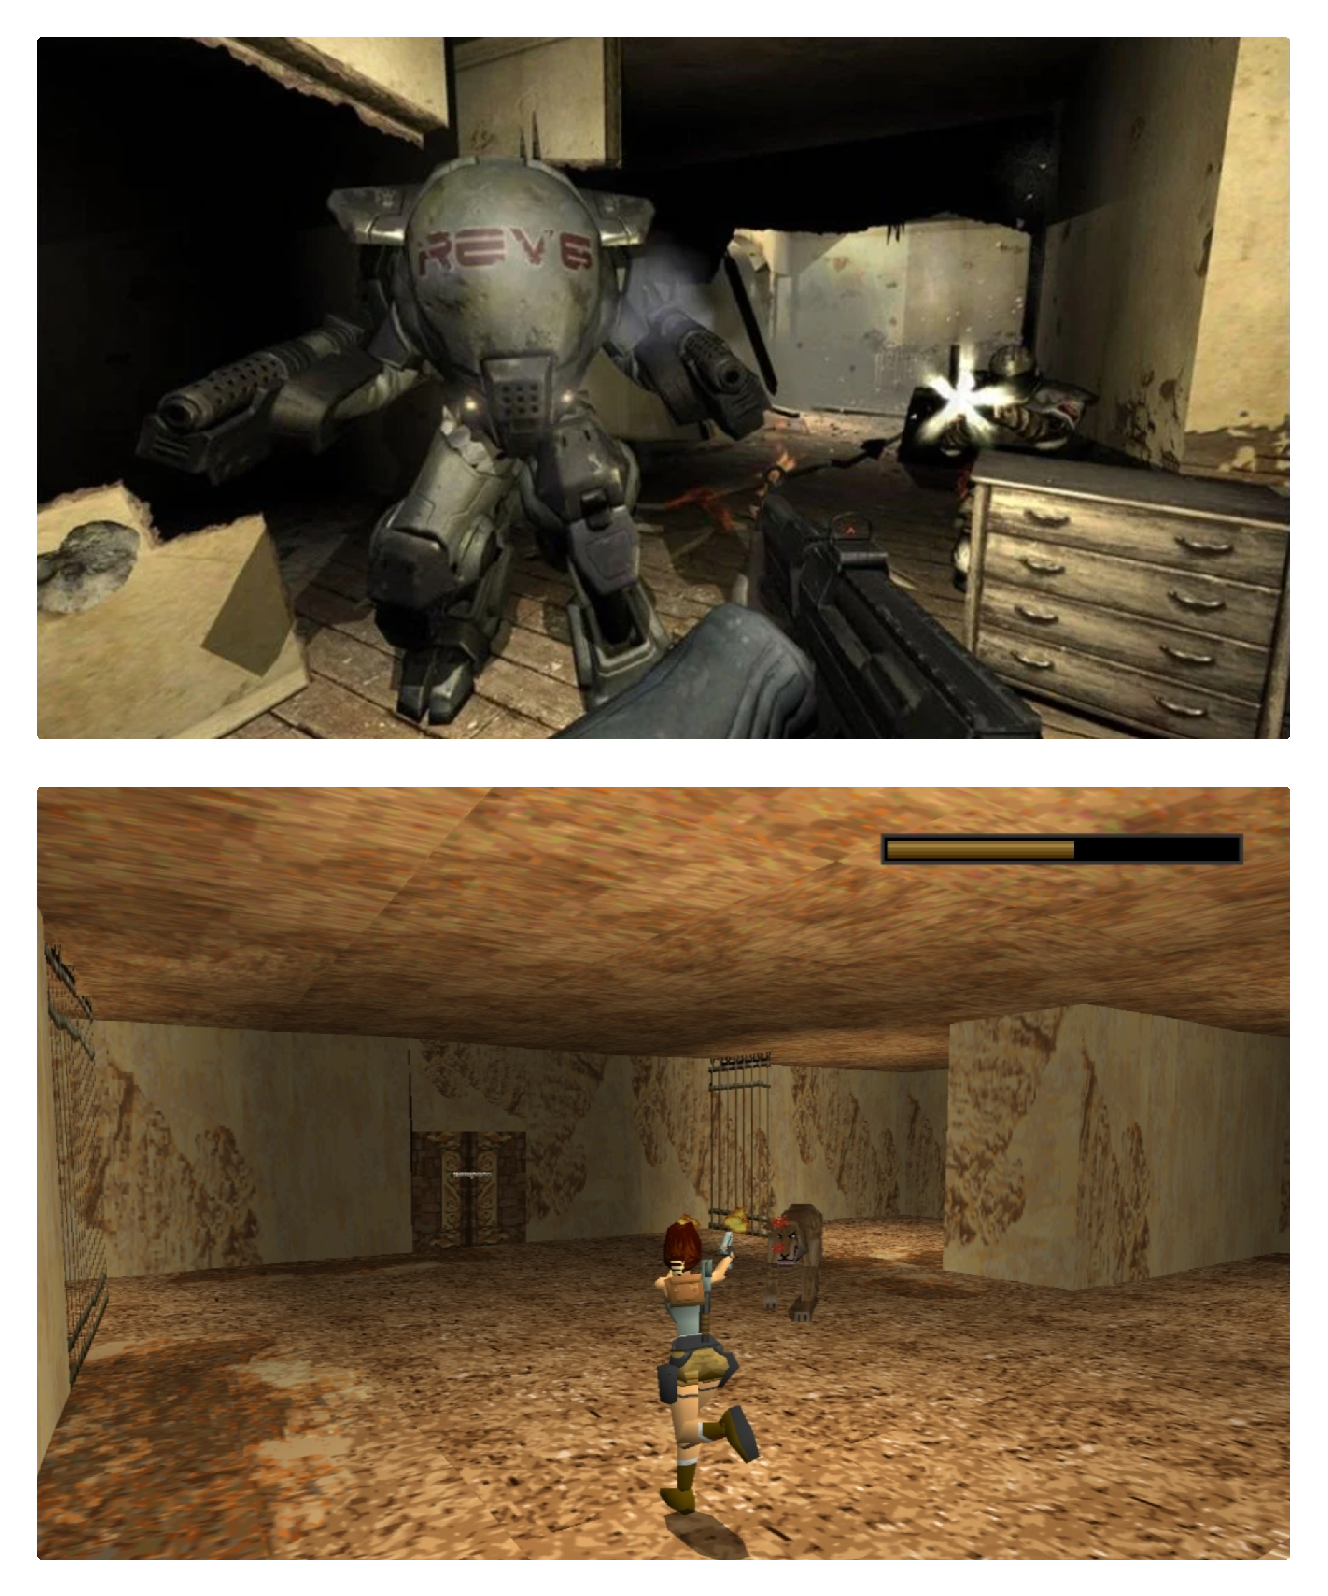
\includegraphics[width=\textwidth]{Videospiele/fps tps}
	\captionsetup{justification=justified, format=plain}
  \caption{First Person Shooter F.E.A.R (links) und Third Person Shooter Tomb Raider (rechts)}
  \label{fig:game-ai model}
\end{figure}


